\documentclass[11pt]{article}
\usepackage[english,vietnam]{babel}
\usepackage[utf8]{inputenc}
\usepackage{a4wide,amssymb,epsfig,latexsym,multicol,array,hhline,fancyhdr}
\usepackage{lastpage}
\usepackage{enumerate}
\usepackage{color}
\usepackage{graphicx}
\usepackage{array}
\usepackage{tabularx}
\usepackage{multirow}
\usepackage{multicol}
\usepackage{rotating}
\usepackage{graphics}
\usepackage[a4paper,left=2cm,right=2cm,top=1.8cm,bottom=2.8cm]{geometry}
\usepackage{setspace}
\usepackage{epsfig}
\usepackage{tikz}
\usepackage{placeins}
\usepackage{appendix}
\usepackage{booktabs}
\usetikzlibrary{arrows,snakes,backgrounds}
\usepackage{amsmath}
\usepackage{listings}
\usepackage{mathtools}
\DeclarePairedDelimiter\ceil{\lceil}{\rceil}
\DeclarePairedDelimiter\floor{\lfloor}{\rfloor}
\usepackage{indentfirst}
\usepackage{titlesec}
\setcounter{secnumdepth}{4}

\title{Assignment Problem For Scheduling TVHS}
\author{Thinh .Q Nguyen \textit{et al.}}
\date{July 2015}

\lstset{
language=C,
basicstyle=\small\sffamily,
frame=tb,
columns=fullflexible,
showstringspaces=false
}

\begin{document}

\begin{titlepage}
\begin{flushleft}
\noindent Trường Đai Học Bách Khoa Tp. Hồ Chí Minh\\
Khoa Khoa Học \& Kỹ Thuật Máy Tính\\
\end{flushleft}

\vspace{1cm}

\begin{figure}[h!]
\begin{center}

\includegraphics[width=30mm]{hcmut.png}
\end{center}
\end{figure}

\vspace{1cm}


\begin{center}
\begin{tabular}{c}
\multicolumn{1}{l}{
\textbf{{\Large AZSHOP}}
}\\
~~\\
\hline
\\
\textbf{{\Huge TÀI LIỆU HƯỚNG DẪN SỬ DỤNG}}\\
\textbf{{\Huge   PHẦN MỀM AZREPORT}}\\
\\
\hline
\end{tabular}
\end{center}

\vspace{3cm}

\begin{minipage}[t]{0.60\linewidth}
\,
\end{minipage}
\begin{minipage}[t]{0.40\linewidth}
Người viết:\\
Nguyễn Quốc Thịnh
\end{minipage}\end{titlepage}

\newpage

\tableofcontents %summary insertion

\newpage
\section{Giới thiệu phần mềm}

\indent Lập lịch cho chương trình quảng cáo là công việc đòi hỏi nhiều thời gian và công sức. Người lập lịch cần biết rất nhiều thông tin về lịch chiếu, chương trình chiếu và doanh số bán hàng, để từ đó đưa ra quyết định sẽ trình chiếu sản phẩm nào vào thời điểm nào. Nhận thấy những khó khăn đó, phần mềm được viết ra nhằm thực hiện các mục tiêu sau:
\begin{itemize}
	\item Cho phép lưu trữ một cách thống nhất các dữ liệu liên quan đến quá trình lập lịch.
	\item Phần mềm có thể tính toán và đưa ra các kết quả thống kê hổ trợ cho người ra quyết định.
	\item Đề xuất lịch chiếu cho người sử dụng.
\end{itemize}
\indent Hiện tại phần mềm chú trọng thực hiện mục tiêu thứ nhất. Các mục tiêu còn lại sẽ hiện thực trong phiên bản tiếp theo.

\section{Các tính năng hiện có của phần mềm}

\subsection{Tính năng nhập danh sách các chương trình quảng cáo}
\indent Tính năng này cho phép người dùng nhập danh sách chương trình quảng cáo bằng file excel (.xls, .xlsx).\\
\begin{figure}[h!]
	\begin{center}
		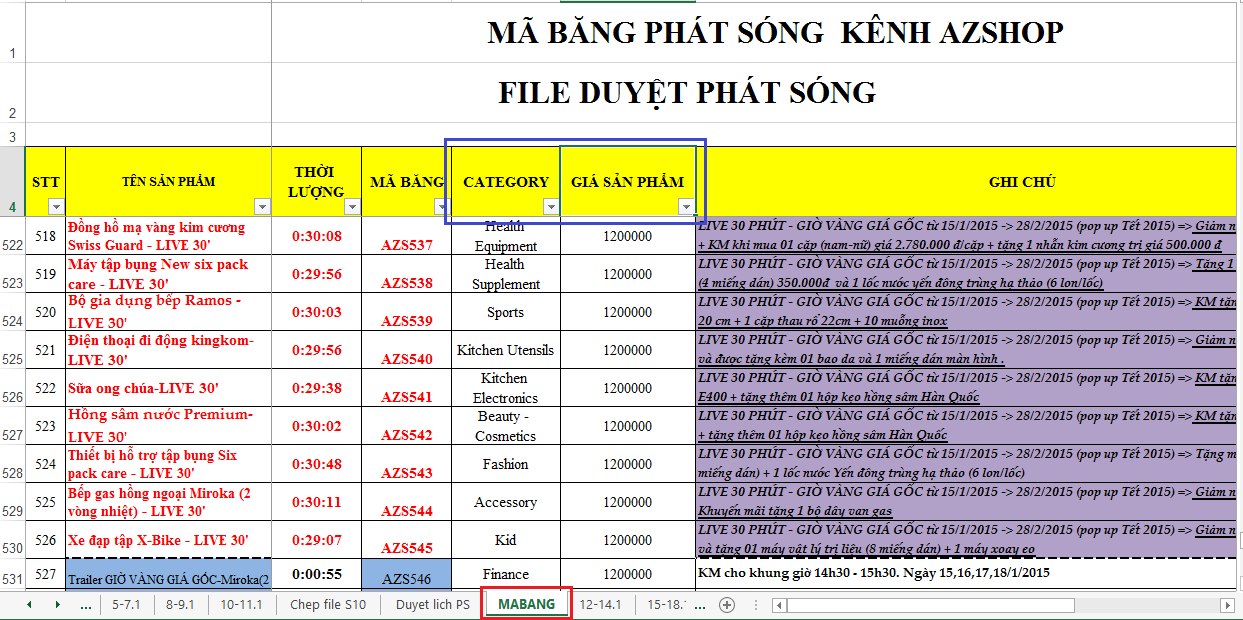
\includegraphics[width=17cm]{mabang.png}
	\end{center}
	\caption{Sheet Bảng Mã}
	\label{bangma}
\end{figure}
\indent So với sheet bảng mã hiện tại thì sheet mới sẽ giữ nguyên tên là "MABANG" đồng thời bổ sung thêm 2 cột mới là "CATEGORY" và " GIÁ SẢN PHẨM".

Giao diện của tính năng như hình \ref{program}. Để thực hiện tính năng chúng ta làm như sau:
\begin{itemize}
	\item Nhấn vào nút Search để tìm file chứa sheet mã băng
	\item Nhấn nút Import để phần mềm lưu lại kết quả từ file.
	\item Checkbox Update được dùng khi người dùng muốn update lại thông tin những chương trình đã từng được lưu trước đó. Trong trường hợp chỉ muốn lưu các chương trình mới thì không chọn vào checkbox này.
\end{itemize}

\begin{figure}[h!]
\begin{center}
	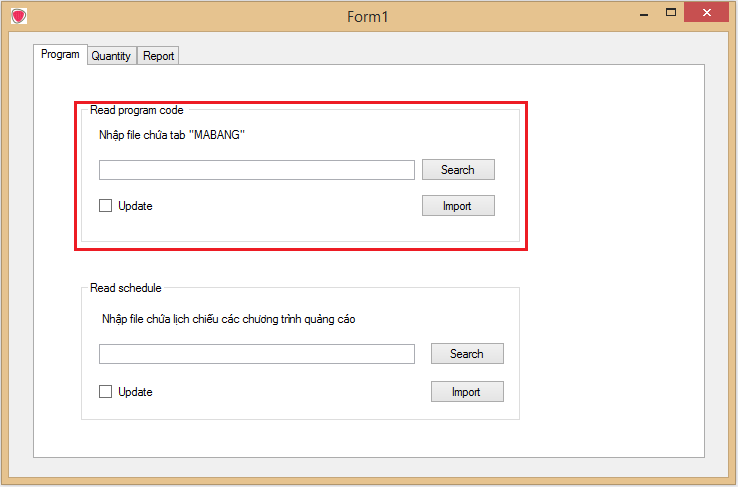
\includegraphics[width=15cm]{program.png}
\end{center}
\caption{Nhập chương trình quảng cáo}
\label{program}
\end{figure}

\subsection{Tính năng nhập lịch đã trình chiếu}
\indent Lịch đã trình chiếu là lịch đã được đưa cho đài truyền hình. Với lịch trình chiếu để phần mềm có thể đọc được cần chú ý một số điểm sau:
\begin{itemize}
	\item Tên và tiêu đề của các sheet tuân theo format như hình \ref{scheduleformat}.
	\begin{figure}[h!]
		\begin{center}
			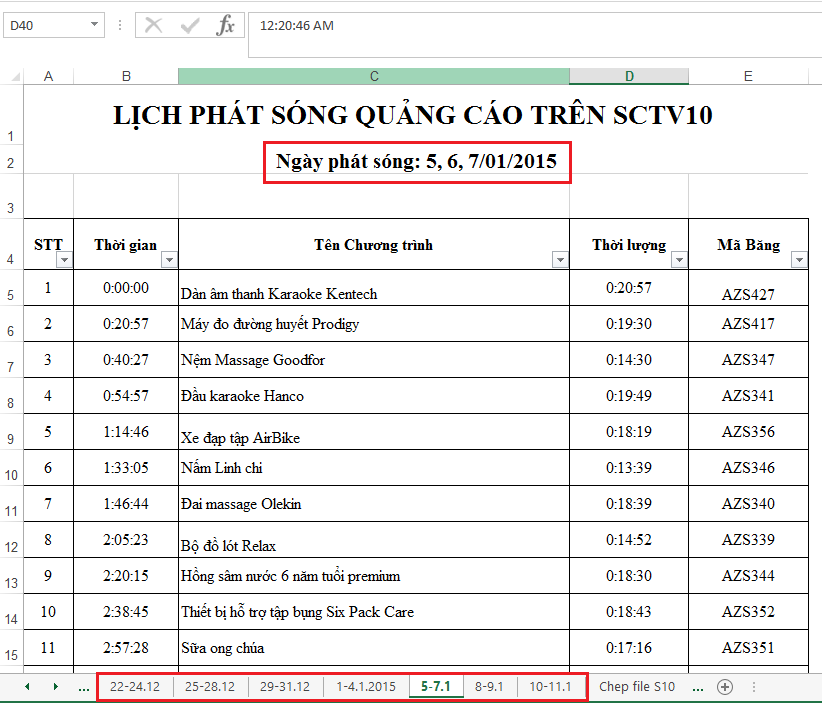
\includegraphics[width=15cm]{scheduleformat.png}
		\end{center}
		\caption{Định dạng tên sheet file và tiêu đề}
		\label{scheduleformat}
	\end{figure}
	\item Nếu tên của sheet không tuân theo format, chương trình sẽ bỏ qua nó.
\end{itemize}

\indent Giao diện của tính năng như hình \ref{schedule}.\\
\begin{figure}[h!]
	\begin{center}
		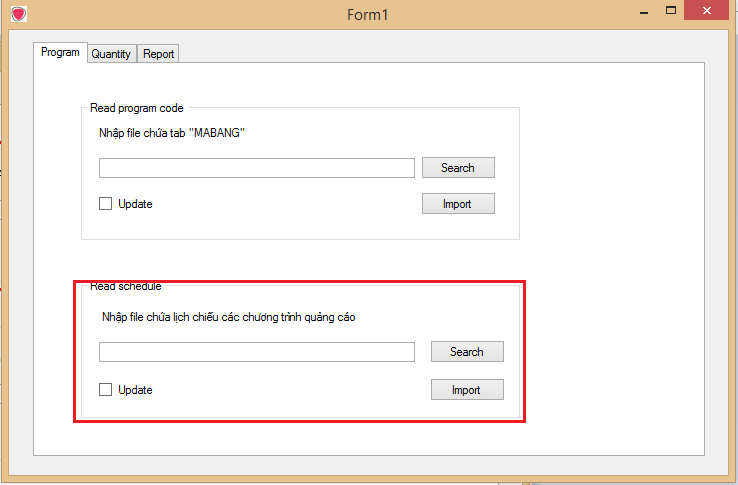
\includegraphics[width=15cm]{schedule.png}
	\end{center}
	\caption{Lịch trình chiếu}
	\label{schedule}
\end{figure}

\indent Cách sử dụng tương tự như tính năng nhập các chương trình quảng cáo.
\subsection{Tính năng tạo mẫu sản lượng bán hàng}
\indent Tính năng này cho phép người dùng định ra khoảng thời gian muốn nhập hoặc xem về thông tin sản lượng bán hàng. Tính năng này trong tab "Quantity" như hình \ref{exquantity}.\\
\begin{figure}[h!]
	\begin{center}
		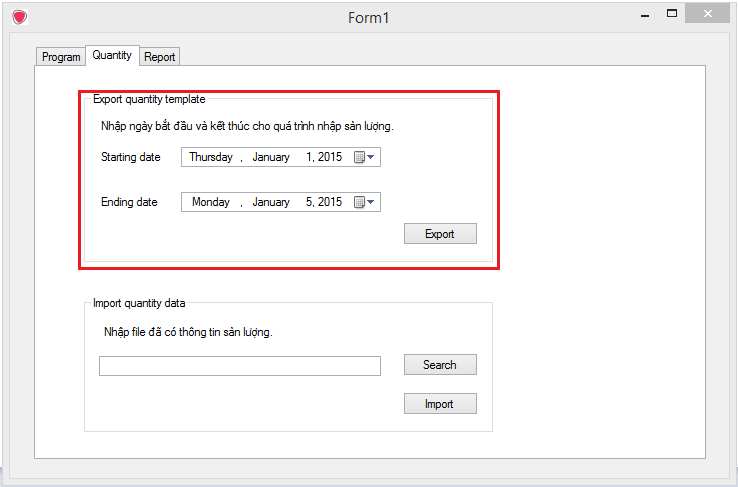
\includegraphics[width=15cm]{exquantity.png}
	\end{center}
	\caption{Tạo mẫu sản lượng bán hàng}
	\label{exquantity}
\end{figure}
\indent Để sử dụng tính năng chúng ta nhập ngày bắt đầu và kết thúc cho phần mềm, sau đó nhấn nút "Export" đề xuất ra mẫu sản lượng bán hàng như hình \ref{mauquantity}.\\
\begin{figure}[h!]
	\begin{center}
		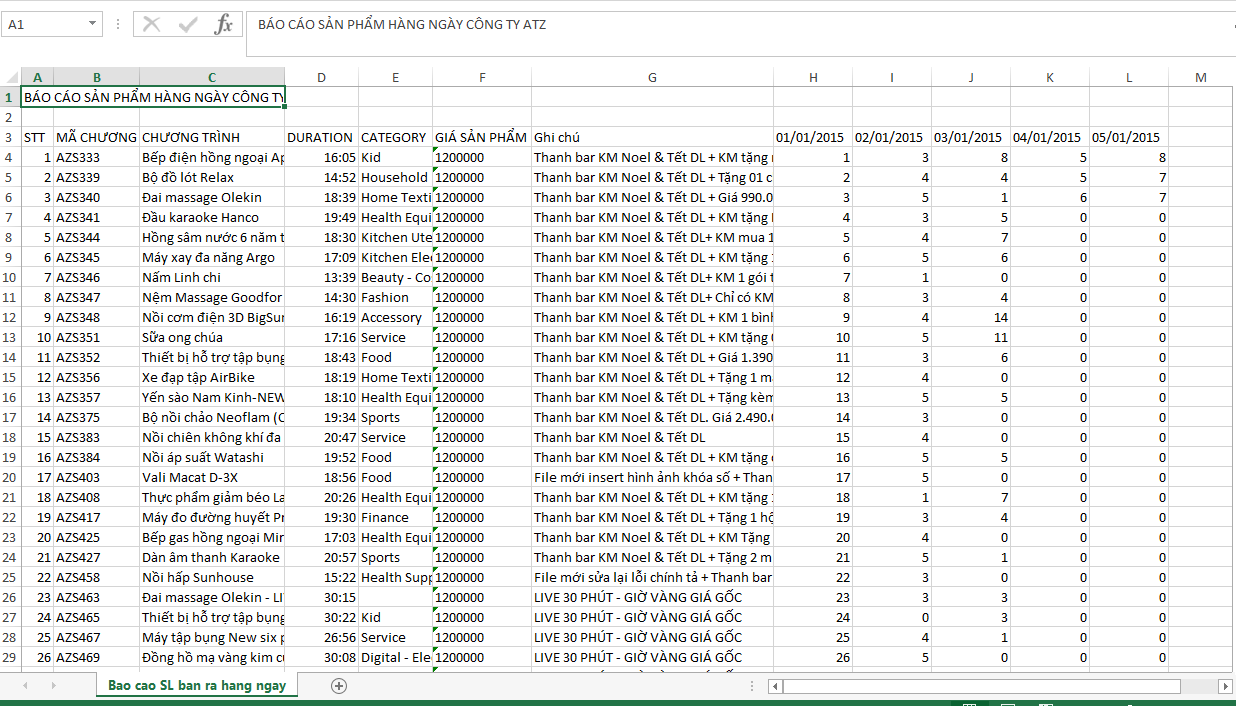
\includegraphics[width=15cm]{mauquantity.png}
	\end{center}
	\caption{Mẫu sản lượng bán hàng}
	\label{mauquantity}
\end{figure}
\subsection{Tính năng lưu sản lượng bán hàng}
\indent Sau khi đã điền thông tin sản lượng vào mẫu sản lượng từ tính năng tạo mẫu sản lượng bán hàng, chúng ta dùng chính file đã tạo để nhập vào tính năng này như hình \ref{imquantity}
\begin{figure}[h!]
	\begin{center}
		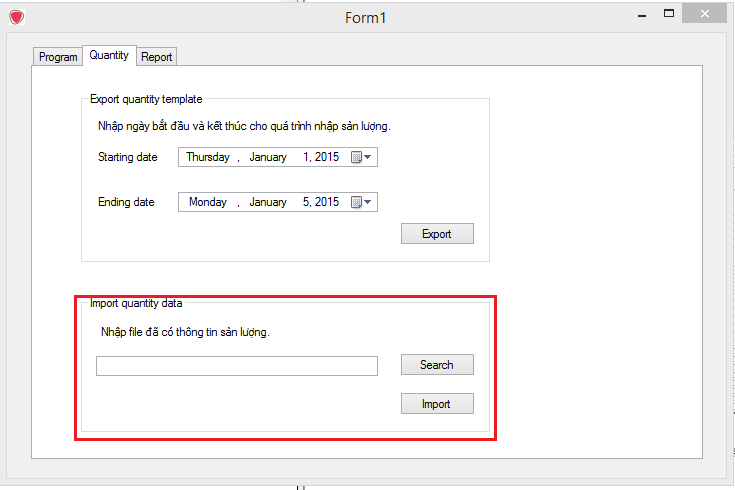
\includegraphics[width=15cm]{imquantity.png}
	\end{center}
	\caption{Lưu sản lượng bán hàng}
	\label{imquantity}
\end{figure}
\indent Nhấn nút Import để nhập dữ liệu bán hàng.
\subsection{Tính năng tạo báo cáo}
\indent Để sử dụng tính năng này chúng ta cần cấu hình trước:
\begin{itemize}
	\item Ngưởng đánh giá cho nhóm sàn phầm (A, B, C), trong khung màu đỏ
	\item Thời gian xét độ hiệu quả, trong khung màu xanh 
\end{itemize}
\begin{figure}[h!]
	\begin{center}
		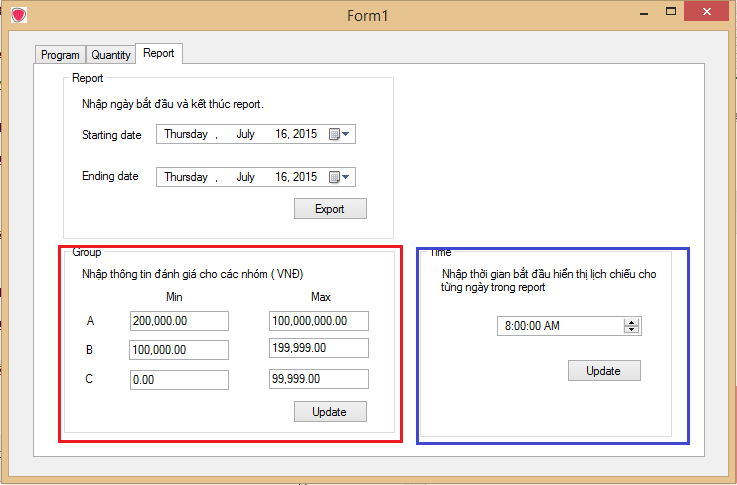
\includegraphics[width=15cm]{report.png}
	\end{center}
	\caption{Báo cáo}
	\label{report}
\end{figure}
\indent Như hình \ref{report}, chúng ta có thể thấy khu vực để xuất report yêu cầu ngày bắt đầu và kết thúc cho báo cáo. Sau khi nhập đầy đủ thông tin nhấn nút Export để xuất ra báo cáo.
\section{Thông báo lỗi}
\indent Khi phần mềm có lỗi, người dùng cần làm những việc sau:
\begin{itemize}
	\item chụp lại màn hình báo lỗi một cách rõ ràng.
	\item miêu tả và cung cấp một cách rõ ràng dữ liệu như thế nào thì gây lỗi cho phần mềm.
	\item Cuối cùng, thông báo cho người viết để sữa lổi.
\end{itemize}
\end{document}
